\chapter{A bivariate beta distribution}
\label{appendix:bivariate-beta-distribution}

\textcite{olkin2015constructions} describe a bivariate distribution with beta
marginal distributions, positive probability over the space $[0,1] \times
[0,1]$, and correlations over the full range $(-1,1)$. In this section, we
derive it and analyse some of its consequences as prior distribution. 

\section{Construction of the distribution}

Let $U = (U_1, U_2, U_3, U_4) \sim
\operatorname{Dirichlet}(\boldsymbol{\alpha})$, where $\boldsymbol{\alpha} =
(\alpha_1, \alpha_2, \alpha_3, \alpha_4)$ with $\alpha_i > 0, i = 1,\dots,4$
and $U_4 = 1 - U_1 + U_2 + U_3$. The joint density of $U$ with respect to the
Lebesgue measure is given by
\begin{equation}
  f_U(u_1, u_2, u_3) = \frac{1}{B(\boldsymbol{\alpha})}u_1^{\alpha_1-1}u_2^{\alpha_2-1}u_3^{\alpha_3-1}(1-u_1-u_2-u_3)^{\alpha_4-1}, 
\end{equation}
when $u_i \in [0,1], i = 1,2,3$, $u_1 + u_2 + u_3 \le 1$, and $0$ otherwise.
The normalizing constant is defined for $\boldsymbol{v} \in \R^n$ as
$$B(\boldsymbol{v}) = \frac{\prod_{i=1}^n \Gamma(v_i)}{\Gamma\left(\sum_{i=1}^n v_i\right)}.$$ 
\begin{definition}
  Let 
  \begin{equation}
    X = U_1 + U_2 \text{ and } Y = U_1 + U_3.
  \end{equation} 
    The distribution of $(X,Y)$ is {\em bivariate beta} with parameter
    $\boldsymbol{\alpha}$. 
\end{definition}

\autoref{fig:beta-bivariate} presents the joint density of $X$ and $Y$ for
different values of $\boldsymbol{\alpha}$. The following two propositions describe the marginal and joint
densities of
bivariate beta distribution.

\begin{figure}[!ht]
  \centering
  \caption{Joint density of the variables $X$ and $Y$ for different choices of $\boldsymbol{\alpha}$.}
  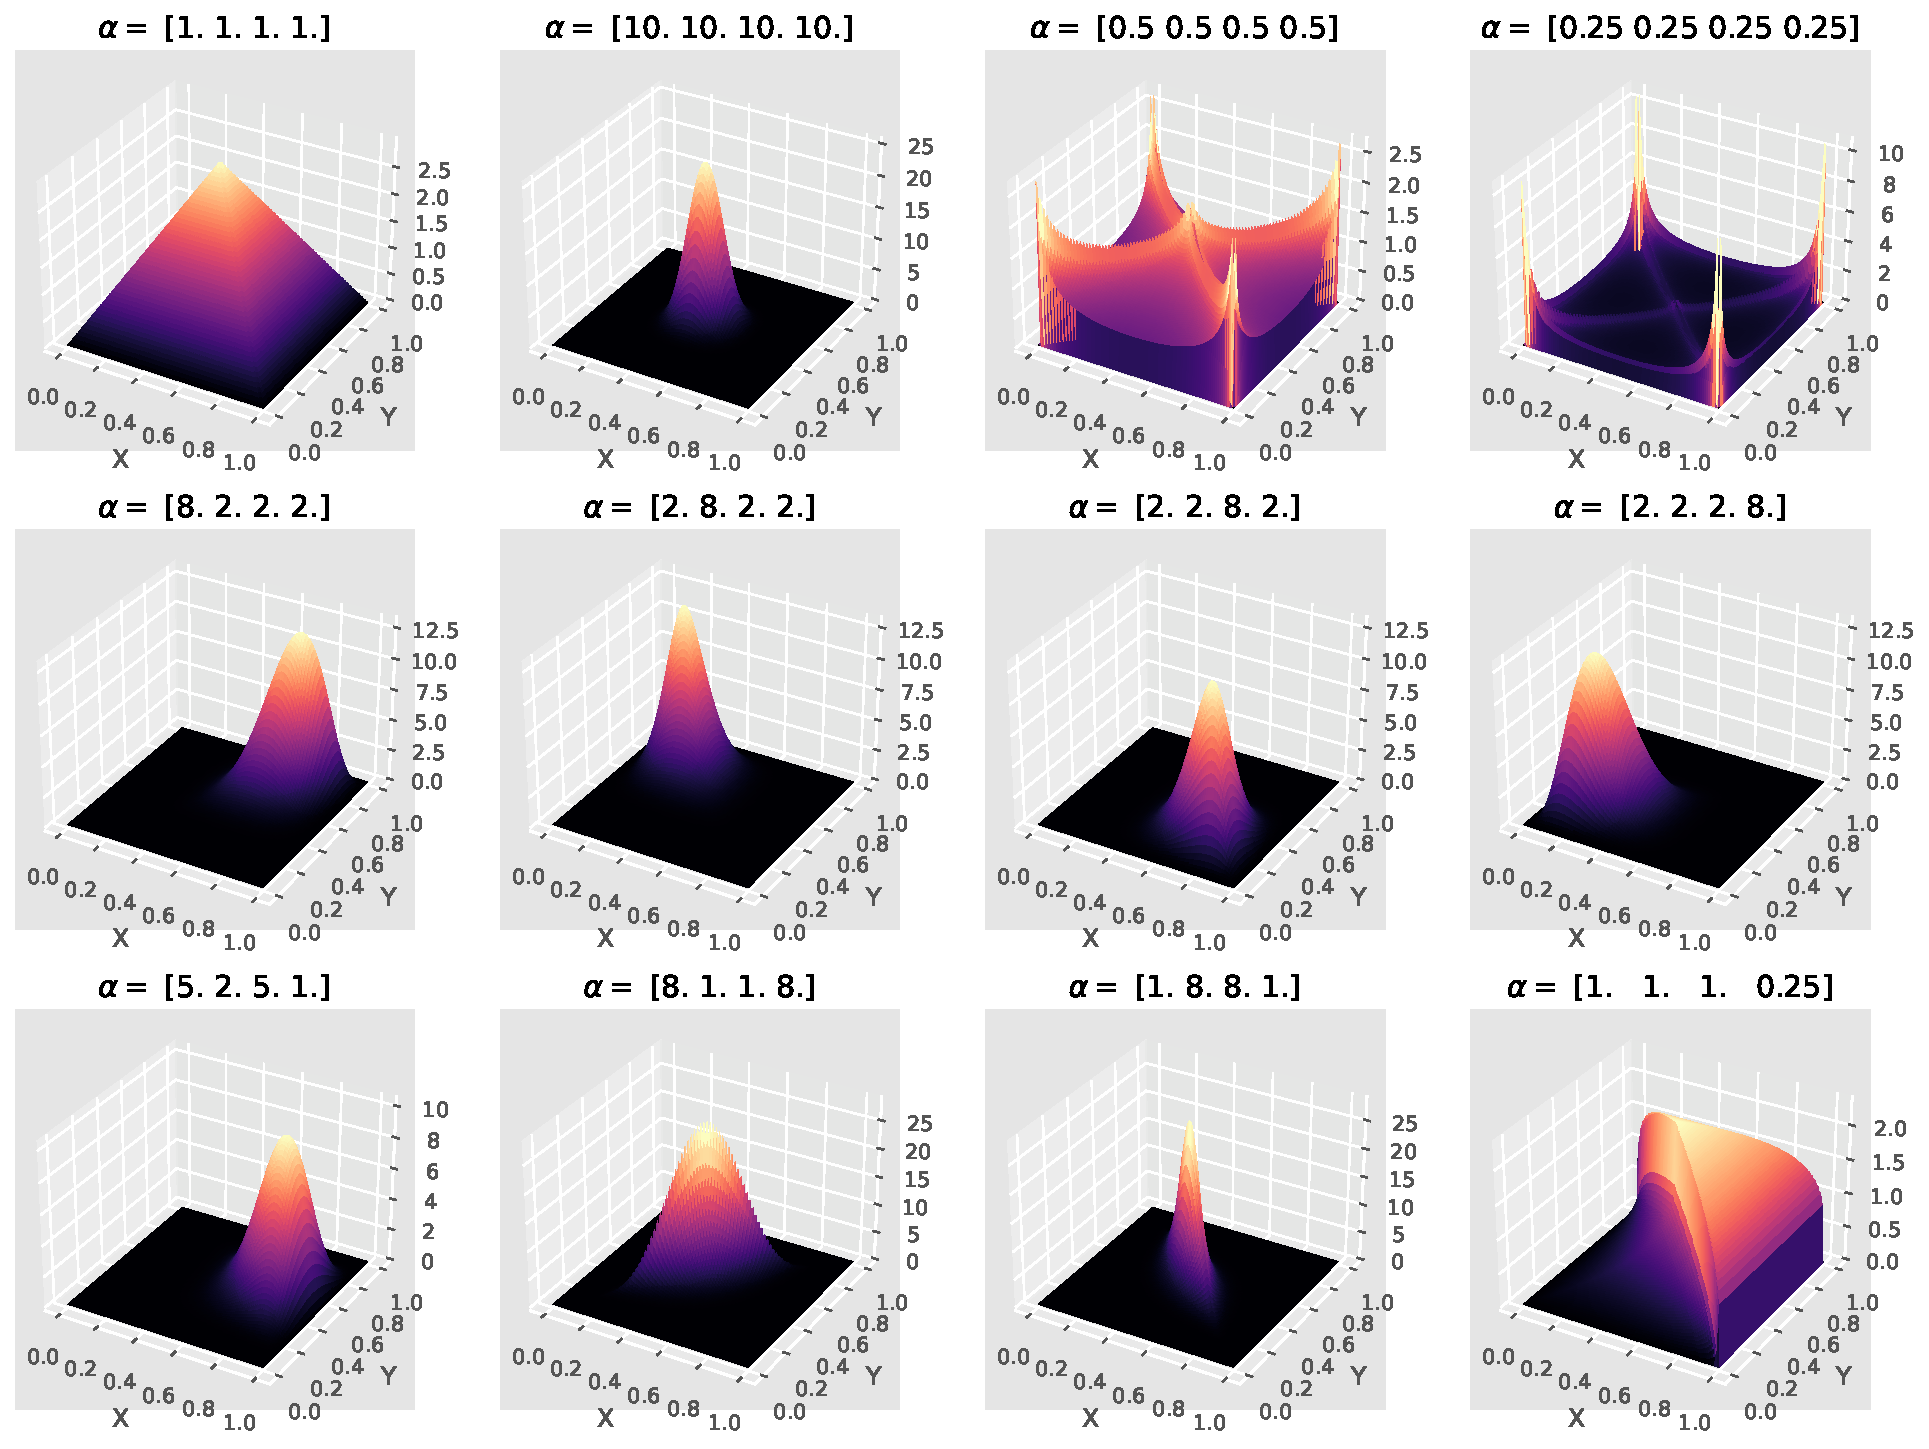
\includegraphics[width=14cm]{joint-densities-bivariate-beta.pdf}
  \fonte{Prepared by the author (2021). The four plots} in the first plot are
  symmetric and have no correlation between the variables. When $\alpha =
  [0.5, 0.5, 0.5, 0.5]$
  \label{fig:beta-bivariate}
\end{figure}

\begin{proposition}[Marginal distributions]
  \label{prop:marginal-distributions}
  The marginal distribution of $X$ is Beta with parameters $\alpha_1 +
  \alpha_2$ and $\alpha_3 + \alpha_4$. Similarly, the marginal distribution of
  $Y$ is Beta with parameters $\alpha_1 + \alpha_3$ and $\alpha_2 + \alpha_4$.
\end{proposition}

\begin{proof}
  First we derive the probability density of $(U_1, U_2)$.
  \begin{equation}
    \label{eq:dist-u1-u2}
    \begin{split}
      f_{U_1, U_2}(u_1, u_2) &= \int_{-\infty}^{\infty} f_{U}(u_1,u_2,u_3) \, du_3 \\ 
      &= \frac{1}{B(\boldsymbol{\alpha})}\int_0^1 u_1^{\alpha_1-1}u_2^{\alpha_2-1}u_3^{\alpha_3-1}(1-u_1-u_2-u_3)^{\alpha_4-1} \, du_3 \\
      &= \frac{1}{B(\boldsymbol{\alpha})}u_1^{\alpha_1-1}u_2^{\alpha_2-1}\int_0^1 u_3^{\alpha_3-1}(1-u_1-u_2-u_3)^{\alpha_4-1} \, du_3.
    \end{split}
  \end{equation}
  Let $u_3 = (1 - u_1 - u_2)z$. Then,
  \begin{equation}
    \begin{split}
      f_{U_1, U_2}(u_1, u_2) &= \frac{1}{B(\boldsymbol{\alpha})}u_1^{\alpha_1-1}u_2^{\alpha_2-1} \\
      &\hspace{1cm} \times \int_0^1 (1-u_1-u_2)^{\alpha_3-1}z^{\alpha_3-1}(1-u_1-u_2)^{\alpha_4}(1-z)^{\alpha_4-1} \, dz. \\
      &= \frac{1}{B(\boldsymbol{\alpha})}u_1^{\alpha_1-1}u_2^{\alpha_2-1}(1-u_1-u_2)^{\alpha_3+\alpha_4-1}\int_0^1 z^{\alpha_3-1}(1-z)^{\alpha_4-1} \, dz. \\
      &= \frac{1}{B(\boldsymbol{\alpha})}u_1^{\alpha_1-1}u_2^{\alpha_2-1}(1-u_1-u_2)^{\alpha_3+\alpha_4-1}\frac{\Gamma(\alpha_3)\Gamma(\alpha_4)}{\Gamma(\alpha_3 + \alpha_4)} \\
      &= \frac{1}{B(\alpha_1, \alpha_2, \alpha_3+\alpha_4)}u_1^{\alpha_1-1}u_2^{\alpha_2-1}(1-u_1-u_2)^{\alpha_3+\alpha_4-1}.
    \end{split}
  \end{equation}

We conclude that
$$(U_1, U_2, 1-U_1-U_2) \sim
\operatorname{Dirichlet}(\alpha_1,\alpha_2,\alpha_3+\alpha_4).$$

Define 
$$
H(v) = \begin{bmatrix}
  1 & 0 \\ 1 & 1
\end{bmatrix}v, \text{ for } v \in \R^2.
$$

Then $(U_1, X) = H(U_1, U_2)$ and $H(\cdot)$ is bijective and differentiable function. By the Change of Variable Formula, 
\begin{equation}
  \begin{split}
    f_{U_1, X}(u_1, x) &= f({H^{-1}(u_1,x)})\bigg|\det\left[\frac{dH^{-1}(v)}{dv}\bigg|_{v=(u_1,x)}\right]\bigg| \\ 
    &= f(u_1, x - u_1) = \frac{1}{B(\alpha_1, \alpha_2, \alpha_3+\alpha_4)}u_1^{\alpha_1-1}(x-u_1)^{\alpha_2-1}(1-x)^{\alpha_3+\alpha_4-1}, 
  \end{split}
\end{equation}
where $(u_1, x)$ belongs to the triangle defined by the points (0,0),
(0,1), and (1,1). The distribution of $X$ for $x \in [0,1]$ is
\begin{equation}
  \begin{split}
    f_X(x) &= \frac{1}{B(\alpha_1, \alpha_2, \alpha_3+\alpha_4)}\int_{0}^{x} u_1^{\alpha_1-1}(x-u_1)^{\alpha_2-1}(1-x)^{\alpha_3+\alpha_4-1} \, du_1 \\
    &= \frac{1}{B(\alpha_1, \alpha_2, \alpha_3+\alpha_4)}(1-x)^{\alpha_3+\alpha_4-1} \int_{0}^{x} u_1^{\alpha_1-1}(x-u_1)^{\alpha_2-1} \, du_1. \\
    &= \frac{1}{B(\alpha_1, \alpha_2, \alpha_3+\alpha_4)}(1-x)^{\alpha_3+\alpha_4-1} \\
    &\hspace{1cm}\times \int_{0}^{x} x^{\alpha_1-1} \left(\frac{u_1}{x}\right)^{\alpha_1-1}x^{\alpha_2 - 1}\left(1-\frac{u_1}{x}\right)^{\alpha_2-1} \, du_1. \\
  \end{split}
\end{equation}

Setting $u = u_1/x$ (if $x = 0, f_X(x) = 0$, then suppose $x > 0$), we have, 
\begin{equation}
  \begin{split}
    f_X(x) &= \frac{1}{B(\alpha_1, \alpha_2, \alpha_3+\alpha_4)}(1-x)^{\alpha_3+\alpha_4-1} x^{\alpha_1+\alpha_2-1} \int_{0}^{1} u^{\alpha_1-1}(1-u)^{\alpha_2-1} \, du. \\
    &= \frac{1}{B(\alpha_1, \alpha_2, \alpha_3+\alpha_4)}(1-x)^{\alpha_3+\alpha_4-1} x^{\alpha_1+\alpha_2-1} B(\alpha_1, \alpha_2)\\
    &= \frac{1}{B(\alpha_1 + \alpha_2, \alpha_3+\alpha_4)}(1-x)^{\alpha_3+\alpha_4-1} x^{\alpha_1+\alpha_2-1}\\
  \end{split}
\end{equation}
Therefore $X \sim \betadist(\alpha_1+\alpha_2, \alpha_3+\alpha_4)$. Similarly $Y \sim \betadist(\alpha_1+\alpha_3, \alpha_2 + \alpha_4)$.
\end{proof}

From the marginal distributions, we already know the expected values and variances of the random variables $X$ and $Y$. Denote $\tilde{\alpha} = \sum_{i=1}^4 \alpha_i$ and we have 

\begin{gather}
    \begin{aligned}
    \ev[X] &= \frac{\alpha_1 + \alpha_2}{\tilde{\alpha}},
    & \ev[Y] &= \frac{\alpha_1 + \alpha_3}{\tilde{\alpha}},
    \\
    \var[X] &= \frac{(\alpha_1 + \alpha_2)(\alpha_3 + \alpha_4)}{\tilde{\alpha}^2(\tilde{\alpha} + 1)},
    & \var[Y] &= \frac{(\alpha_1 + \alpha_3)(\alpha_2 + \alpha_4)}{\tilde{\alpha}^2(\tilde{\alpha} + 1)}.
    \end{aligned}
\end{gather}

\begin{proposition}[Bivariate beta density]
  \label{prop:bivariate-beta-density}
  The joint density of $(X,Y)$ with respect to the Lebesgue measure is
  given by 
  \begin{equation}
    f_{X,Y}(x,y) = \frac{1}{B(\boldsymbol{\alpha})}\int_{\Omega} u_1^{\alpha_1 - 1}(x - u_1)^{\alpha_2 -1}(y-u_1)^{\alpha_3-1}(1-x-y+u_1)^{\alpha_4-1} \, du_1,
  \end{equation}
  where 
  $$
  \Omega = (\max(0, x+y-1), \min(x,y)).
  $$
\end{proposition}

\begin{proof}
  Note that
  $$
  \begin{bmatrix}
    U_1 \\ X \\ Y
  \end{bmatrix}  = \begin{bmatrix}
    1 & 0 & 0 \\
    1 & 1 & 0 \\
    1 & 0 & 1
  \end{bmatrix}\begin{bmatrix}
    U_1 \\ U_2 \\ U_3
  \end{bmatrix}, 
  $$
  where the linear function is bijective and differentiable function, such
  that the determinant of the derivative is 1. By the Change of Variable
  Formula, 
  \begin{equation}
    \begin{split}
      f_{U_1,X,Y}(u_1,x,y) &= f_{U_1,U_2,U_3}(u_1, x - u_1, y - u_2) \\ 
      &= \frac{1}{B(\boldsymbol{\alpha})}u_1^{\alpha_1-1}(x-u_1)^{\alpha_2-1}(y-u_1 )^{\alpha_3-1}(1-x-y+u_1)^{\alpha_4-1},
    \end{split}
  \end{equation}
  where $0 \le u_1 \le x, u_1 \le y$, and $0 \le 1 - x - y + u_1$.  
  Hence,
  \begin{equation}
      \label{eq:dist-X-Y}
      f_{X,Y}(x,y) = \frac{1}{B(\boldsymbol{\alpha})}\int_{\Omega} u_1^{\alpha_1-1}(x-u_1)^{\alpha_2-1}(y-u_1)^{\alpha_3-1}(1-x-y+u_1)^{\alpha_4-1} \, du_1,
  \end{equation}
  such that $\Omega = \{u_1 : \max(0, x + y -1) < u_1 < \min(x,y)\}$.
\end{proof}

At last we derive the covariance and the correlation between $X$ and $Y$.

\begin{proposition}[Covariance and correlation]
  \label{prop:covariance-correlation}
  The covariance between $X$ and $Y$ is 
  $$\cov(X,Y) = \frac{1}{\tilde{\alpha}^2(\tilde{\alpha}+1)}(\alpha_1\alpha_4 - \alpha_2\alpha_3)$$
  and
  $$\cor(X,Y) = \frac{\alpha_1\alpha_4 - \alpha_2\alpha_3}{\sqrt{(\alpha_1+\alpha_2)(\alpha_3+\alpha_4)(\alpha_1+\alpha_3)(\alpha_2+\alpha_4)}}.$$
\end{proposition}

\begin{proof}

  The covariance between $U_i$ and $U_j$ is \cite[p. 11]{lin2016dirichlet} 
\begin{equation}
  \cov(U_i, U_j) = - \frac{\alpha_i\alpha_j}{\tilde{\alpha}^2(\tilde{\alpha}+1)}, i,j = 1,...,4, i \neq j
\end{equation} 
and the variance of $U_i$ is 
\begin{equation}
  \var(U_i) = \frac{\alpha_i(\tilde{\alpha}-\alpha_i)}{\tilde{\alpha}^2(\tilde{\alpha}+1)},
\end{equation}
since $U_i \sim \operatorname{Beta}(\alpha_i, \tilde{\alpha} -\alpha_i)$.
Therefore 
\begin{equation}
  \cov(X,Y) = \cov(U_1+U_2, U_1+U_3) = \frac{1}{\tilde{\alpha}^2(\tilde{\alpha}+1)}(\alpha_1\alpha_4 - \alpha_2\alpha_3).
\end{equation}
  
\end{proof}

Now we present an example where the full range of correlation is covered.
Suppose $X$ and $Y$ have uniform distribution over $[0,1]$, that is, they have
beta distribution with parameter $1,1$. Then, we have that 
$$\alpha_1 +
\alpha_2 = \alpha_3 + \alpha_4 = \alpha_1 + \alpha_3 = \alpha_2 + \alpha_4 = 1,$$
whose solution is $\alpha_1 = \alpha_4 \in (0,1)$ and $\alpha_2 = \alpha_3 = 1
- \alpha_4$. The correlation formula boils down to 
$$\cor(X,Y) = \alpha_4^2 - (1 - \alpha_4)^2 = 2\alpha_4 - 1 \in (-1,1).$$

\section{Implementation of the dirichlet distribution in Stan}

The Dirichlet distribution is defined on the simplex of lower dimension.
Therefore the sampler has to consider the restriction of $\sum_{i=1}^4 U_i =
  1$. \textcite{betancourt2012cruising} presents a simplification in the
structure of the simplex. The propose is \cite[p. 2]{betancourt2012cruising}
\begin{equation*}
  \begin{aligned}
    z_i & \sim \betadist(\tilde{\alpha}_i, \alpha_i), \text{ where } \tilde{\alpha}_i = \sum_{k=i+1}^4 \alpha_k, \quad i = 1,2,3 \\
    U_i & = \left(\prod_{k=1}^{i-1} z_k\right)\cdot \begin{cases}
      1 - z_i, & i < 4 \\
      1,       & i = 4
    \end{cases},
  \end{aligned}
\end{equation*}
which removes the constraint.

\section{Comments about integration}

The density of $(X,Y)$ is $f_{X,Y}(x,y)$ as in equation \eqref{eq:dist-X-Y} and it can be undefined in sets of null Lebesgue measure in $\R^2$ and these sets may be important when plotting in a grid, for instance. This section illustrates one of these sets. If $\alpha_i \ge 1,
\, i = 1,...,4$, the integral is clearly well defined for every $x,y \in [0,1]$. Let $0 < \alpha_2 = \alpha_3 = a \le 0.5$ and $x = y < 0.5$. Then
\begin{equation*}
  \begin{split}
    f_{X,Y}(x,y) &= \frac{1}{B(\boldsymbol{\alpha})}\int_{0}^x u_1^{\alpha_1-1}(x-u_1)^{a-1}(x-u_1)^{a-1}(1-2x+u_1)^{\alpha_4-1} \, du_1 \\
    &= \frac{1}{B(\boldsymbol{\alpha})}\int_{0}^{x/2} u_1^{\alpha_1-1}(x-u_1)^{2a-2}(1-2x+u_1)^{\alpha_4-1} \, du_1 + \\
    &~~~+ \frac{1}{B(\boldsymbol{\alpha})}\int_{x/2}^x u_1^{\alpha_1-1}(x-u_1)^{2a-2}(1-2x+u_1)^{\alpha_4-1} \, du_1
  \end{split}
\end{equation*}

Note that the first integral is well defined and non-negative. On the other hand, the second integral is not defined: 
\begin{equation*}
  \begin{split}
    \int_{x/2}^{x} u_1^{\alpha_1-1}&(x-u_1)^{2a-2}(1-2x+u_1)^{\alpha_4-1} \, du_1 \\
    &\ge \int_{x/2}^x \min\left(\left(\frac{x}{2}\right)^{\alpha_1-1}, x^{\alpha_1-1}\right)(x-u_1)^{2a-2} \\ 
    &\hspace{3cm} \times \min\left(\left(1-\frac{3}{2}x\right)^{\alpha_4-1}, (1-x)^{\alpha_4-1}\right) \, du_1 \\
    &= K(x) \int_{0}^{x/2} v^{2a-2} \, dv \\ 
    &= \begin{cases}
      \dfrac{K(x)}{2a-1} \lim_{t \to 0^+} \left[(x/2)^{2a-1} - t^{2a-1}\right] &\text{ if } a < 0.5 \\ 
      K(x) \lim_{t \to 0^+} \left[\log(x/2) - \log(t)\right] &\text{ if } a = 0.5
    \end{cases} \\
    &\to +\infty, 
  \end{split}
\end{equation*}
where $K(x)$ is a function of $x$. 

Based on this divergence, we conclude that if $0 < \alpha_2 = \alpha_3 \le 0.5$
and $x = y < 0.5$, $f_{X,Y}(x,y)$ is not defined. Notice that if $x = y \ge
0.5$, divergence problems still happens, since the problems appear when $u_1$ approximates $x$. Similar calculations show that if $x + y = 1$ and $0 < \alpha_1 = \alpha_4 \le 0.5$, the density is also
not defined. More generally, $f_{X,Y}(x,y)$ is not defined if $\alpha_1 +
\alpha_4 \le 1$ and $x + y = 1$; $\alpha_2 + \alpha_3 \le 1$ and $x = y$.

\section{Elicitation of a bivariate beta}
\label{sec:elicitation-bivariate-beta}

In this section, we develop a method to elicit the parameters of the bivariate
beta distribution, which means to define an approximation
$\hat{\boldsymbol{\alpha}}$ for the parameter $\boldsymbol{\alpha}$. 
This is an important step for the characterization of the prior distribution of model
\eqref{model:sensitivity-specificity}. If the researcher does not have
information about the parameters previous seeing the data, two approaches
are common in the independent beta setting and are adapted for the bivariate 
case:

\begin{alineas}
  \item both parameters receive a uniform distribution: in this case, as
  mentioned in Proposition \ref{prop:covariance-correlation}, $\alpha_1 =
  \alpha_4 \in (0,1)$ and $\alpha_2 = \alpha_3 = 1 - \alpha_4$. The parameter
  $\alpha_4$ is defined in a way that $\alpha_4 = \frac{1}{2}(1 + \cor(X,Y))$.
  If no information about the variables' correlation is available, it is recommended to use
  the independent setting since it is more flexible;
  \item both parameters receive a Jeffreys' prior distribution
  ($\betadist(1/2,1/2)$): in this case,  $\alpha_1 =
  \alpha_4 \in (0,1/2)$ and $\alpha_2 = \alpha_3 = 1 - \alpha_4$. The parameter
  $\alpha_4$ is defined in a way that $\alpha_4 = \frac{1}{4}(1 + \cor(X,Y))$.
\end{alineas}

Now, suppose that the researcher has information about following moments of
the bivariate beta distribution: $m_1 = \ev[X], m_2 = \ev[Y], v_1 = \var(X),
v_2 = \var(Y)$, and $\rho  = \cor(X,Y)$. Notice that $v_1 + m_1^2 = \var(X_1)
+ \ev[X_1]^2 = \ev[X_1^2]$ and
$$
\ev[X_1^2] - \ev[X_1] = \frac{(\alpha_1 + \alpha_2 + 1)(\alpha_1 + \alpha_2)}{(\tilde{\alpha} + 1)\tilde{\alpha}} - \frac{\alpha_1 + \alpha_2}{\tilde{\alpha}} = -\frac{(\alpha_1 + \alpha_2)(\alpha_3 + \alpha_4)}{\tilde{\alpha}(\tilde{\alpha}+1)} < 0, 
$$
that is, $v_1 + m_1^2 - m_1 < 0 \implies v_1 < m_1 - m_1^2$ and similarly,
$v_2 < m_2 - m_2^2$. After fixing these quantities, we will have a non-linear system with five equations and four
unknown variables. Hence, we want to solve the following 
\begin{equation}
  \label{eq:system-moments-alpha}
  \begin{cases}
    m_1 = \dfrac{\alpha_1+\alpha_2}{\tilde{\alpha}}, \\
    m_2 = \dfrac{\alpha_1+\alpha_3}{\tilde{\alpha}}, \\ 
    v_1 = \dfrac{(\alpha_1+\alpha_2)(\alpha_3+\alpha_4)}{\tilde{\alpha}^2(\tilde{\alpha}+1)}, \\
    v_2 = \dfrac{(\alpha_1+\alpha_3)(\alpha_2+\alpha_4)}{\tilde{\alpha}^2(\tilde{\alpha}+1)}, \\
    \rho = \dfrac{\alpha_1\alpha_4 - \alpha_2\alpha_3}{\sqrt{(\alpha_1+\alpha_2)(\alpha_3+\alpha_4)(\alpha_1+\alpha_3)(\alpha_2+\alpha_4)}}.
  \end{cases}
\end{equation}

Notice that we can simplify the third and fourth equations since 
$$
\frac{\alpha_3 + \alpha_4}{\tilde{\alpha}} = \frac{\tilde{\alpha} - (\alpha_1 + \alpha_2)}{\tilde{\alpha}} = 1 - m_1, 
$$
and analogously, 
$$
\frac{\alpha_2 + \alpha_4}{\tilde{\alpha}} = 1 - m_2. 
$$
Therefore, 
\begin{align*}
    v_1 &= \frac{m_1(1 - m_1)}{\tilde{\alpha} + 1}, \\
    v_2 &= \frac{m_2(1 - m_2)}{\tilde{\alpha} + 1}.
\end{align*}

This already tells us that the system do not have a solution if 
$$
\frac{m_1(1-m_1)}{v_1} \neq \frac{m_2(1-m_2)}{v_2}. 
$$

The following proposition builds a solution excluding the fourth equation, given the above comment. 

\begin{proposition}
  \label{prop:solution-to-system-bivariate-beta}
  System \eqref{eq:system-moments-alpha} without the fourth equation has a unique solution given by 
\begin{gather}
 \label{eq:system-solution}
 \begin{aligned}
  \alpha_1 &= (m_1 + m_2 - 1)\tilde{\alpha} + \alpha_4, \\
  \alpha_2 &=  (1 - m_2)\tilde{\alpha} - \alpha_4, \\
  \alpha_3 &= (1-m_1)\tilde{\alpha} - \alpha_4, \\
  \alpha_4 &= \rho\tilde{\alpha}\sqrt{m_1m_2(1-m_1)(1-m_2)} + (1-m_1)(1-m_2),
\end{aligned}
\end{gather}
where $\tilde{\alpha}$ is given by the expression 
$$
\tilde{\alpha} = \frac{(m_1 - m_1^2 - v_1)}{v_1}.
$$
\end{proposition}

\begin{proof}
  The first two equations of the system \eqref{eq:system-moments-alpha} can be
rewritten as a linear system:
\begin{align*}
  (m_1 - 1)\alpha_1 + (m_1 - 1)\alpha_2 + m_1\alpha_3 + m_1\alpha_4 &= 0, \\
  (m_2 - 1)\alpha_1 + m_2\alpha_2 + (m_2-1)\alpha_3 + m_2\alpha_4 &= 0,   
\end{align*}
which is equivalent to 
\begin{align*}
  \alpha_1 + \alpha_2 + \frac{m_1}{m_1-1}\alpha_3 + \frac{m_1}{m_1-1}\alpha_4 &= 0, \\
  \alpha_2 + \frac{1-m_2}{m_1-1}\alpha_3 + \frac{m_1-m_2}{m_1-1}\alpha_4 &= 0.
\end{align*}
Then, we can write $\alpha_1$ and $\alpha_2$ as functions of $\alpha_3$ and
$\alpha_4$:
\begin{align}
  \label{eq:alpha1-as-function-alpha3-alpha4}
  \alpha_1 &= \frac{m_1+m_2-1}{1-m_1}\alpha_3 + \frac{m_2}{1-m_1}\alpha_4 \\
  \label{eq:alpha2-as-function-alpha3-alpha4}
  \alpha_2 &= \frac{1-m_2}{1-m_1}\alpha_3 + \frac{m_1-m_2}{1-m_1}\alpha_4.
\end{align}

Based on that expression, denote $\alpha_1 = a_3\alpha_3 + a_4\alpha_4$, $\alpha_2
= b_3\alpha_3 + b_4\alpha_4$, $c_3 = a_3 + b_3 + 1$, and $c_4 = a_4 + b_4 + 1$. Then, the third equation can be written as 
$$
a_3\alpha_3 + a_4\alpha_4 + b_3\alpha_3 + b_4\alpha_4 + \alpha_3 + \alpha_4 + 1 = c_3\alpha_3 + c_4 \alpha_4 = \frac{m_1(1-m_1)}{v_1} - 1, 
$$
which implies that 
$$
\alpha_3 = \frac{m_1(1-m_1) - v_1 - c_4v_1\alpha_4}{c_3v_1},
$$
that is a linear function of $\alpha_4$. We summarize the expressions in function of $\alpha_4$ with some simplifications: 
\begin{align*}
  \alpha_1 &= (m_1 + m_2 - 1)\frac{(m_1 - m_1^2 - v_1)}{v_1} + \alpha_4, \\
  \alpha_2 &=  (1 - m_2)\frac{(m_1 - m_1^2 - v_1)}{v_1} - \alpha_4, \\
  \alpha_3 &= (1-m_1)\frac{(m_1 - m_1^2 - v_1)}{v_1} - \alpha_4,
\end{align*}
which implies that 
$$
\tilde{\alpha} = \frac{m_1 - m_1^2 - v_1}{v_1}.
$$

Now rewrite the fifth equation using the first two equations from system \eqref{eq:system-moments-alpha} as follows 
\begin{equation}
    \label{eq:rho-equation}
    \begin{split}
        \rho &= \frac{\alpha_1\alpha_4 - \alpha_2\alpha_3}{\sqrt{(\alpha_1+\alpha_2)(\alpha_3+\alpha_4)(\alpha_1+\alpha_3)(\alpha_2+\alpha_4)}} \\ 
        &= \frac{\alpha_1\alpha_4 - \alpha_2\alpha_3}{\tilde{\alpha}^2\sqrt{m_1m_2(1-m_1)(1-m_2)}} \\ 
        &= \frac{(m_1 + m_2 - 1)\tilde{\alpha}\alpha_4 + \alpha_4^2 - ((1-m_2)\tilde{\alpha} - \alpha_4)((1-m_1)\tilde{\alpha} - \alpha_4)}{\tilde{\alpha}^2\sqrt{m_1m_2(1-m_1)(1-m_2)}} \\
        &= \frac{\alpha_4 - (1-m_1)(1-m_2)\tilde{\alpha}}{\tilde{\alpha}\sqrt{m_1m_2(1-m_1)(1-m_2)}} \\ 
    \end{split}
\end{equation}
and the solution is, therefore, 
$$
\alpha_4 = \rho\tilde{\alpha}\sqrt{m_1m_2(1-m_1)(1-m_2)} + (1-m_1)(1-m_2).
$$
\end{proof}

There is an additional restriction to the sum given by the marginal
distributions. Let $Z \sim \betadist(a, b)$. Then: 
$$
\frac{\ev[Z](1-\ev[Z])}{\var[Z]} - 1 = \frac{\frac{ab}{(a+b)^2}}{\frac{ab}{(a+b)^2(a+b+1)}}-1 = a+b, 
$$
then 
\begin{equation}
  \label{eq:restriction-sum-alphas}
  \sum_{i=1}^4 \alpha_i = \frac{m_1(1-m_1)}{v_1} - 1 = \frac{m_2(1-m_2)}{v_2} - 1.
\end{equation}

Besides solving the system \eqref{eq:system-moments-alpha}, the bivariate 
beta distribution needs that $\alpha_1, \dots, \alpha_4 > 0$. However, this is
not always achievable. Since it is difficult to find the subset $D \subset [0,1]^4$ in
which
the solution for \eqref{eq:system-solution} is strictly positive for
$\alpha_1, \dots, \alpha_4$, we present some examples in Figure
\ref{fig:alpha-solutions}. For each subplot, the values of $v_1$ and $\rho$
are fixed, while $m_1, m_2 \in [0,1]^2$. The grey area corresponds to the set 
where $v_1 \ge m_1 - m_2$, which is impossible. The orange area means that
the solution to system \eqref{eq:system-moments-alpha} is not strictly
positive. At last, the blue region is the set of interest. 

When $\rho = -1$ for instance, only a few specifications of $m_1$ and $m_2$
generate a strictly positive solution. These examples show that several
interesting specifications for the researchers can lead to a non positive
solution, which is not desirable. 

\begin{figure}[!ht]
    \centering
    \caption{Verification of positivity of the solution for different and
    fixed values of $v_1$ and $\rho$, and $m_1, m_2 \in [0,1]^2$.} 
    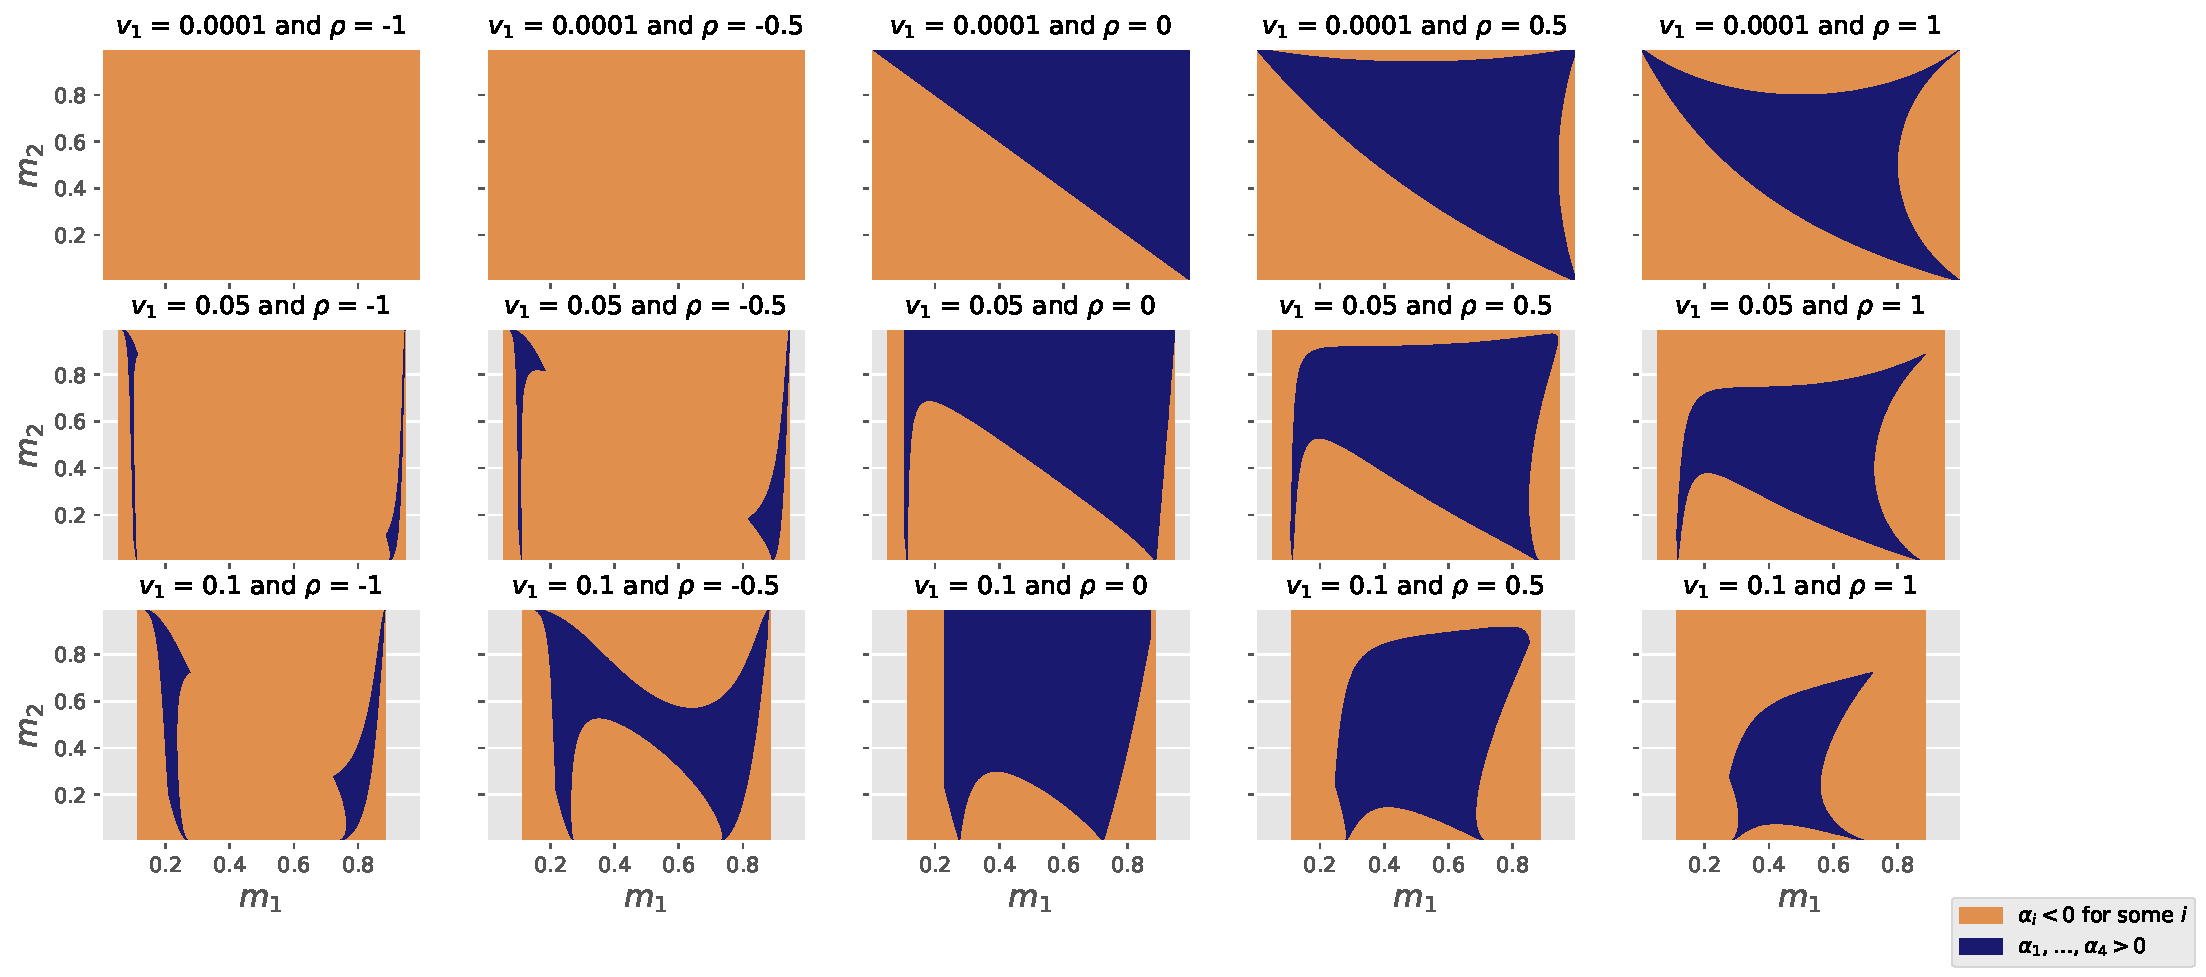
\includegraphics[width=\textwidth]{alpha_solution_existence.pdf}
    \fonte{Prepared by the author (2021).}
    \label{fig:alpha-solutions}
\end{figure}

In light of this, we can only have an approximation using some
optimization solver. From now on, we suppose the researcher has knowledge about
$m_1$, $m_2$ and $\rho$. Through equations
\eqref{eq:alpha1-as-function-alpha3-alpha4}, 
\eqref{eq:alpha2-as-function-alpha3-alpha4}, and solving the correlation
equation for $\alpha_3$ with help of the symbolic solver SymPy \cite{sympy},
we have the following three expressions: 
\begin{equation*}
  \begin{aligned}
    \alpha_1 &= \alpha_4\frac{m_1m_2 + \rho\sqrt{m_1m_2(1-m_1)(1-m_2)}}{(1-m_1)(1-m_2) + \rho\sqrt{m_1m_2(1-m_1)(1-m_2)}}, \\
    \alpha_2 &= \alpha_4\frac{m_1(1-m_2) - \rho\sqrt{m_1m_2(1-m_1)(1-m_2)}}{(1-m_1)(1-m_2) + \rho\sqrt{m_1m_2(1-m_1)(1-m_2)}}, \\
    \alpha_3 &= \alpha_4\frac{m_2(1-m_1) - \rho\sqrt{m_1m_2(1-m_1)(1-m_2)}}{(1-m_1)(1-m_2) + \rho\sqrt{m_1m_2(1-m_1)(1-m_2)}},
  \end{aligned}
\end{equation*}
and $\alpha_4 > 0$ is a free parameter. In order to have $\boldsymbol{\alpha} >
0$, we have two situations:
\begin{alineas}
  \item the denominator of $\alpha_1, \alpha_2, \alpha_3$ is negative: in this
  case, it is not possible to have both $\alpha_2$ and $\alpha_3$ positives;
  \item the denominator of  $\alpha_1, \alpha_2, \alpha_3$ is positive: in
  this case, we have that 
  $$
  \rho \in \left(-\frac{\min(m_1m_2, (1-m_1)(1-m_2))}{\sqrt{m_1m_2(1-m_1)(1-m_2)}}, 
  \frac{\max(m_1, m_2) - m_1m_2}{\sqrt{m_1m_2(1-m_1)(1-m_2)}}\right).
  $$
\end{alineas}

When $m_1 = m_2 = m$, the upper bound is 1 and the lower bound is 
$$\begin{cases}
  -\dfrac{m}{1-m}, &m < 1/2 \\
  -\dfrac{1-m}{m}, &m > 1/2.
\end{cases}$$

Suppose that $\rho$ belongs to this interval. Then we have to choose $\alpha_4
> 0$. Using a symbolic solver, we see that 
$$
\sum_{i=1}^4 \alpha_i = \frac{\alpha_4}{(1-m_1)(1-m_2) + \rho\sqrt{m_1m_2(1-m_1)(1-m_2)}}, 
$$
therefore $v_1$ and $v_2$ are inversely proportional to $\alpha_4$. To have a
higher variance, pick a small $\alpha_4$. To have a lower variance, pick a
large one. If $\rho$ does not belong to the interval, taking a suitable value
in it is a possibility. 

Suppose the researcher has also knowledge about $v_1$ and $v_2$. By
Proposition \ref{prop:solution-to-system-bivariate-beta} and
\autoref{fig:alpha-solutions}, there is no viable
solution in several situations. Because of that, two approaches are suggested:

\begin{alineas}
  \item no variable is fixed: solve the optimizing problem given by 
  \textcite[p. 7]{olkin2015constructions}. The problem with this approach is 
  that $\rho$ and the means $m_1, m_2$ get far from the given values.
  Weights can be specified for each parameter to incorporate some preference;  
  \item fix $m_1$ and $m_2$ and let $\rho, v_1$ and $v_2$ vary: it is the
  limit of the above method, with the weights of $m_1$ and $m_2$ going to the
  infinity. It is more suitable when the researcher has stronger beliefs or information in the
  means than the other moments. 
\end{alineas}

In this work, we use the second approach, which gives less importance to the
correlation in comparison to the means. 

\begin{remark}
  If the researcher has information about a credibility interval, this
  information needs to be converted in terms of the variance for our framework.
\end{remark}

\section{Simulate data}

In this section, we experiment the estimation process of $\hat{\boldsymbol{\alpha}}$ through
two different simulations: 

\begin{alineas}
  \item simulating from bivariate beta: fix the parameter $\alpha = (0.5, 0.5,
  0.5, 0.5)$ and generate $1000$
  different datasets from bivariate beta distribution of size $100$; calculate
  $m_1, m_2, v_1, v_2$, and $\rho$ and (i) solve the equations through Proposition
  \eqref{prop:solution-to-system-bivariate-beta}, (ii) complete optimization
  problem, and (iii) optimization problem with $m_1$ and $m_2$ fixed, which we
  call {\em mixed solver}. The mean squared error is calculated;
  \item simulating from bivariate logit normal distribution: fix the means and
  covariance matrix and follow the same instructions from the previous item.
\end{alineas}

Since the comparison is in terms of mean squared error, it is clear that the
minimization problem will have the least value. When time is important, it is
a very expensive method. Solving equations should be the best method, but
under uncertainty, its results can have biases.
\autoref{tab:comparing-approaches-bivariate-beta} summarizes the results. 
Notice that when simulating from the bivariate beta or from the bivariate
logit normal with parameters corresponding to the beta, the estimation process
has little error. 

\begin{table}[hb]
  \centering
  \caption{\label{tab:comparing-approaches-bivariate-beta}Comparing the
  different methods for each simulation strategy.}
  \begin{tabular}{cccc}
  \hline
  \multicolumn{1}{c}{\textbf{Simulation}} & \textbf{Method} & \textbf{MSE} & \textbf{s/ite} \\ \hline
  \multirow{3}{*}{Bivariate beta} & Solving equations & 0.04 & $3.47 \cdot 10^{-5}$ \\
   & Minimization problem & 0.032 & $1.43$ \\
   & Mixed solver & 0.033 & $0.03$ \\
  \multirow{3}{*}{Logit bivariate normal} & Solving equations & 0.034 & $5.21 \cdot 10^{-5}$ \\
   & Minimization problem & 0.026 & $1.53$ \\
   & Mixed solver & 0.026 & $0.03$  \\ \hline
  \end{tabular}
  \fonte{Prepared by the author (2021). The MSE is the mean squared error,
  where the mean is taken with respect to the iterations. The s/ite is the
  number of seconds per iteration.}
\end{table}

Using the logit bivariate normal simulation with parameters $\mu = (5, 2.3)$
and $\Sigma = [[12, -2.5], [-2.5, 4]]$ in order to yield $\ev[X] \approx 0.9,
\ev[Y] \approx 0.8, \var(X) = \var(Y) \approx 0.05$, and $\cor(X,Y) \approx
-0.2$, 77\% of the simulations has no exact solution strictly positive and the
error of the solvers were 0.82 for the mixed solver and 0.91 for the
minimization problem, which is much higher than the previous simulation.

\chapter{Sampling from the posterior distribution of the graph}
\label{sec:sampling-posterior-graph}

Here we derive the method developed by \textcite{crawford2016} for sampling
from $p(G_S, \lambda \mid \boldsymbol{Z})$. The
implementation used Python language. We first define
the prior density for $(G_s, \lambda)$ as 
$$
\pi(G_S, \lambda) = \pi(G_S) \times \pi(\lambda) = \frac{1}{|\mathcal{C}(\boldsymbol{Z})|} \times \frac{\beta_{r}^{\alpha_{r}}}{\Gamma(\alpha_{r})}\lambda^{\alpha_r - 1}e^{-\beta_r \lambda}, 
$$
where $\alpha_r$ and $\beta_r$ are positive hyperparameters. Notice that $G_S$
as uniform distribution over all compatible graphs and $\lambda \sim
\operatorname{Gamma}(\alpha_r, \beta_r)$.

To perform Gibbs sampling, we need to sample from $p(G_S \mid \lambda,
\boldsymbol{Z})$ and $p(\lambda \mid G_S , \boldsymbol{Z})$. Since we do not
know to sample from both conditional distributions, \textcite{crawford2016}
proposes to use Metropolis-Hastings for each one. Then, we need to specify a
proposal distribution to both conditionals:
\begin{alineas}
  \item the proposal for $p (G_S | \lambda, \boldsymbol{Z})$ generates a new compatible graph
   $G_S^*$ with a simple algorithm. It samples two random nodes $i,j$
   without replacement. If both nodes have less connections in $G_S$ than
   their informed degrees, i.e., $u_i \ge 1$ and
   $u_j \ge 1$, and they are not connected in $G_S$, we include the edge
   $\{i,j\}$ in $G_S^*$ and copy all the other edges. If the edge already is
   in $G_S$ and it is not in $G_R$, we remove it from $G_S^*$. Otherwise we
   draw another two nodes and continue. We call this proposal of $P(G_S^* \mid
   G_S)$; 
   \item the proposal for $p(\lambda \mid G_S, \boldsymbol{Z})$ assumes a
   normal distribution for the Maximum likelihood estimator (MLE)
   $\hat{\lambda}$ of $\lambda$ from the likelihood
   \eqref{eq:likelihood-wainting-times}. Deriving it, we obtain 
   \begin{equation*}
     \begin{split}
      \frac{d}{d \lambda} \log L(w \mid G_S, \lambda) &= \frac{d}{d \lambda}\left[ (n - m)\log(\lambda) + \sum_{k \text{ isn't seed}} \log(s_k) - \lambda \boldsymbol{s}^Tw\right] \\
      &= \frac{n-m}{\lambda} - \boldsymbol{s}^Tw,
     \end{split}
   \end{equation*}
   where $m$ is the number of seeds. At the optimal $\hat{\lambda}$, we have
   that 
   $$
   \frac{n-m}{\hat{\lambda}} - \boldsymbol{s}^Tw = 0 \implies \hat{\lambda} = \frac{n-m}{\boldsymbol{s}^Tw}.
   $$
   The Fisher information is, under some regularity conditions,
   $$
   I(\lambda) = -\ev\left[-\frac{n-m}{\lambda^2}\right] = \frac{n-m}{\lambda^2}.
   $$
   For a large $n$, we can assume
   $$\sqrt{n-m}(\hat{\lambda} - \lambda) \overset{d}{\to} N(0, \lambda^2).$$ 
   Then the proposal distribution is the normal distribution of mean
   $\hat{\lambda}$ and variance $\sigma^2 = \lambda^2/(n - m)$.
\end{alineas} 

Now, it remains to calculate the probability of acceptance for both
Metropolis-Hastings samplings. \textcite{crawford2016} 
establishes several results to make the calculations more efficient. We omit
them here. Using relation \eqref{eq:alpha-metropolis-hastings}, the probabilities are: 

\begin{alineas}
  \item for the graph transition:
  \begin{equation*}
    \begin{split}
      \alpha(G_S^* \mid G_S) &= \min\left(1, \frac{p (G_S^*| \lambda, \boldsymbol{Z})P(G_S \mid G_S^*)}{p (G_S | \lambda, \boldsymbol{Z}) P(G_S^* \mid G_S)}\right) \\
      &= \min\left(1, \frac{L(w \mid G_S^*, \lambda)\pi(G_S^*)\pi(\lambda)P(G_S \mid G_S^*)}{ L(w \mid G_S, \lambda)\pi(G_S)\pi(\lambda)P(G_S^* \mid G_S)}\right) \\
      &= \min\left(1, \frac{L(w \mid G_S^*, \lambda)P(G_S \mid G_S^*)}{ L(w \mid G_S, \lambda)P(G_S^* \mid G_S)}\right);
    \end{split}
  \end{equation*}
  \item for the rate $\lambda$ transition:
  \begin{equation*}
    \begin{split}
      \alpha(\lambda^* \mid \lambda) &= \min\left(1, \frac{p (\lambda^* \mid  G_S,  \boldsymbol{Z})g(\lambda \mid G_S)}{p (\lambda \mid G_S, \boldsymbol{Z}) g(\lambda^* \mid G_S)}\right) \\
      &= \min\left(1, \frac{L(w \mid G_S, \lambda^*)\pi(G_S)\pi(\lambda^*)g(\lambda \mid G_S)}{ L(w \mid G_S, \lambda)\pi(G_S)\pi(\lambda)P(\lambda \mid G_S)}\right) \\
      &= \min\left(1, \frac{L(w \mid G_S, \lambda^*)\pi(\lambda^*)g(\lambda \mid G_S)}{ L(w \mid G_S, \lambda)\pi(\lambda) g(\lambda^* \mid G_S)}\right).
    \end{split}
  \end{equation*}
  This probability is better calculated using the logarithmic transformations,
  since 
  $$
  \log \frac{L(w \mid G_S, \lambda^*)}{ L(w \mid G_S, \lambda)} = (n-m)\left(\log(\lambda^*) - \log(\lambda)\right) - \boldsymbol{s}^Tw(\lambda^* - \lambda),
  $$
  $$
  \log \frac{\pi(\lambda^*)}{\pi(\lambda)} = (\alpha_r - 1)(\log(\lambda^*) - \log(\lambda)) - \beta(\lambda^* - \lambda), \text{ and }
  $$
  $$
  \log \frac{g(\lambda \mid G_S)}{g(\lambda^* \mid G_S)} = \log(\lambda^*) - \log(\lambda) - \frac{1}{2}\left[\frac{(\lambda - \hat{\lambda})^2}{\sigma^2} - \frac{(\lambda^* - \hat{\lambda})^2}{(\sigma^*)^2}\right].
  $$
\end{alineas}

Establishing the Metropolis-Hastings, the Gibbs sampling is well-defined.

\chapter{Stan codes}
\label{appendix:stan-codes}

\section{Perfect tests}

This is the Stan code for model \eqref{model:perfect-tests}

\lstinputlisting[basicstyle=\footnotesize, language=Stan]{../../models/primary_model/stan_codes/perfect_test.stan}

\section{Sensitivity and specificity}

This is the Stan code for model \eqref{model:sensitivity-specificity}

\subsection*{Logit normal prior}

\lstinputlisting[basicstyle=\footnotesize, language=Stan]{../../models/sensitivity_specificity/spec_sens_model_logit_normal.stan}

\subsection*{Bivariate beta prior with constant $\alpha$}

\lstinputlisting[basicstyle=\footnotesize, language=Stan]{../../models/sensitivity_specificity/spec_sens_model_constant_alpha_smooth.stan}

\subsection*{Bivariate beta prior with random $\alpha$}

\lstinputlisting[basicstyle=\footnotesize, language=Stan]{../../models/sensitivity_specificity/spec_sens_model_random_alpha_smooth.stan}

\section{Imperfect tests}

This is the Stan code for model \eqref{model:imperfect-tests}

\lstinputlisting[basicstyle=\footnotesize, language=Stan]{../../models/primary_model/stan_codes/imperfect_test.stan}

\section{Imperfect tests and respondent-driven sampling}

This is the Stan code for model \eqref{model:imperfect-tests-rds}

\lstinputlisting[basicstyle=\footnotesize, language=Stan]{../../models/primary_model/stan_codes/rds_imperfect_test_v5.stan}


